\section{Transactions}
A peer will have transactions with other peers in the network.
The peer will want to have an increase in his reputation and have a transaction be created.
The transaction contains the information about how much data was uploaded and downloaded between the peers
and their total upload and download amounts.

The transaction will be encapsulated inside a single block.
A block contains both public keys of the peers,
so it is possible to see between which peers the transaction is.
Both peers sign the block to acknowledge that the transaction has happened.
Every block only contains one transaction.

The blocks are linked to previous blocks by adding the hashes of the previous blocks of both peers.
This creates a directed acyclic graph of blocks.
A chain can be identified within this graph for every peer.
This chain contains every transaction of a peer.

An example of three blocks can be seen in Figure \ref{fig:chain-example}.
The arrows denote the corresponding hash or signature.
In this example the first block is between peer B and C.
The block contains hashes to the previous blocks of both B and C
and can be seen by the outward arrows.
Inside the block it can be seen what part peer B and C signs by the boxes.
The whole block is not signed by both parties.
The reason for this is explained in section \ref{design:block_creation}.

In the example both peer B and C also conduct a transaction with another peer, A and D respectively.
This creates two new blocks and are chained to the block between B and C by adding the previous hash to the new blocks.
The new blocks also contains the previous hashes of A and D
and chain the new block to previous blocks of A and D.

\begin{figure}
	\centerline{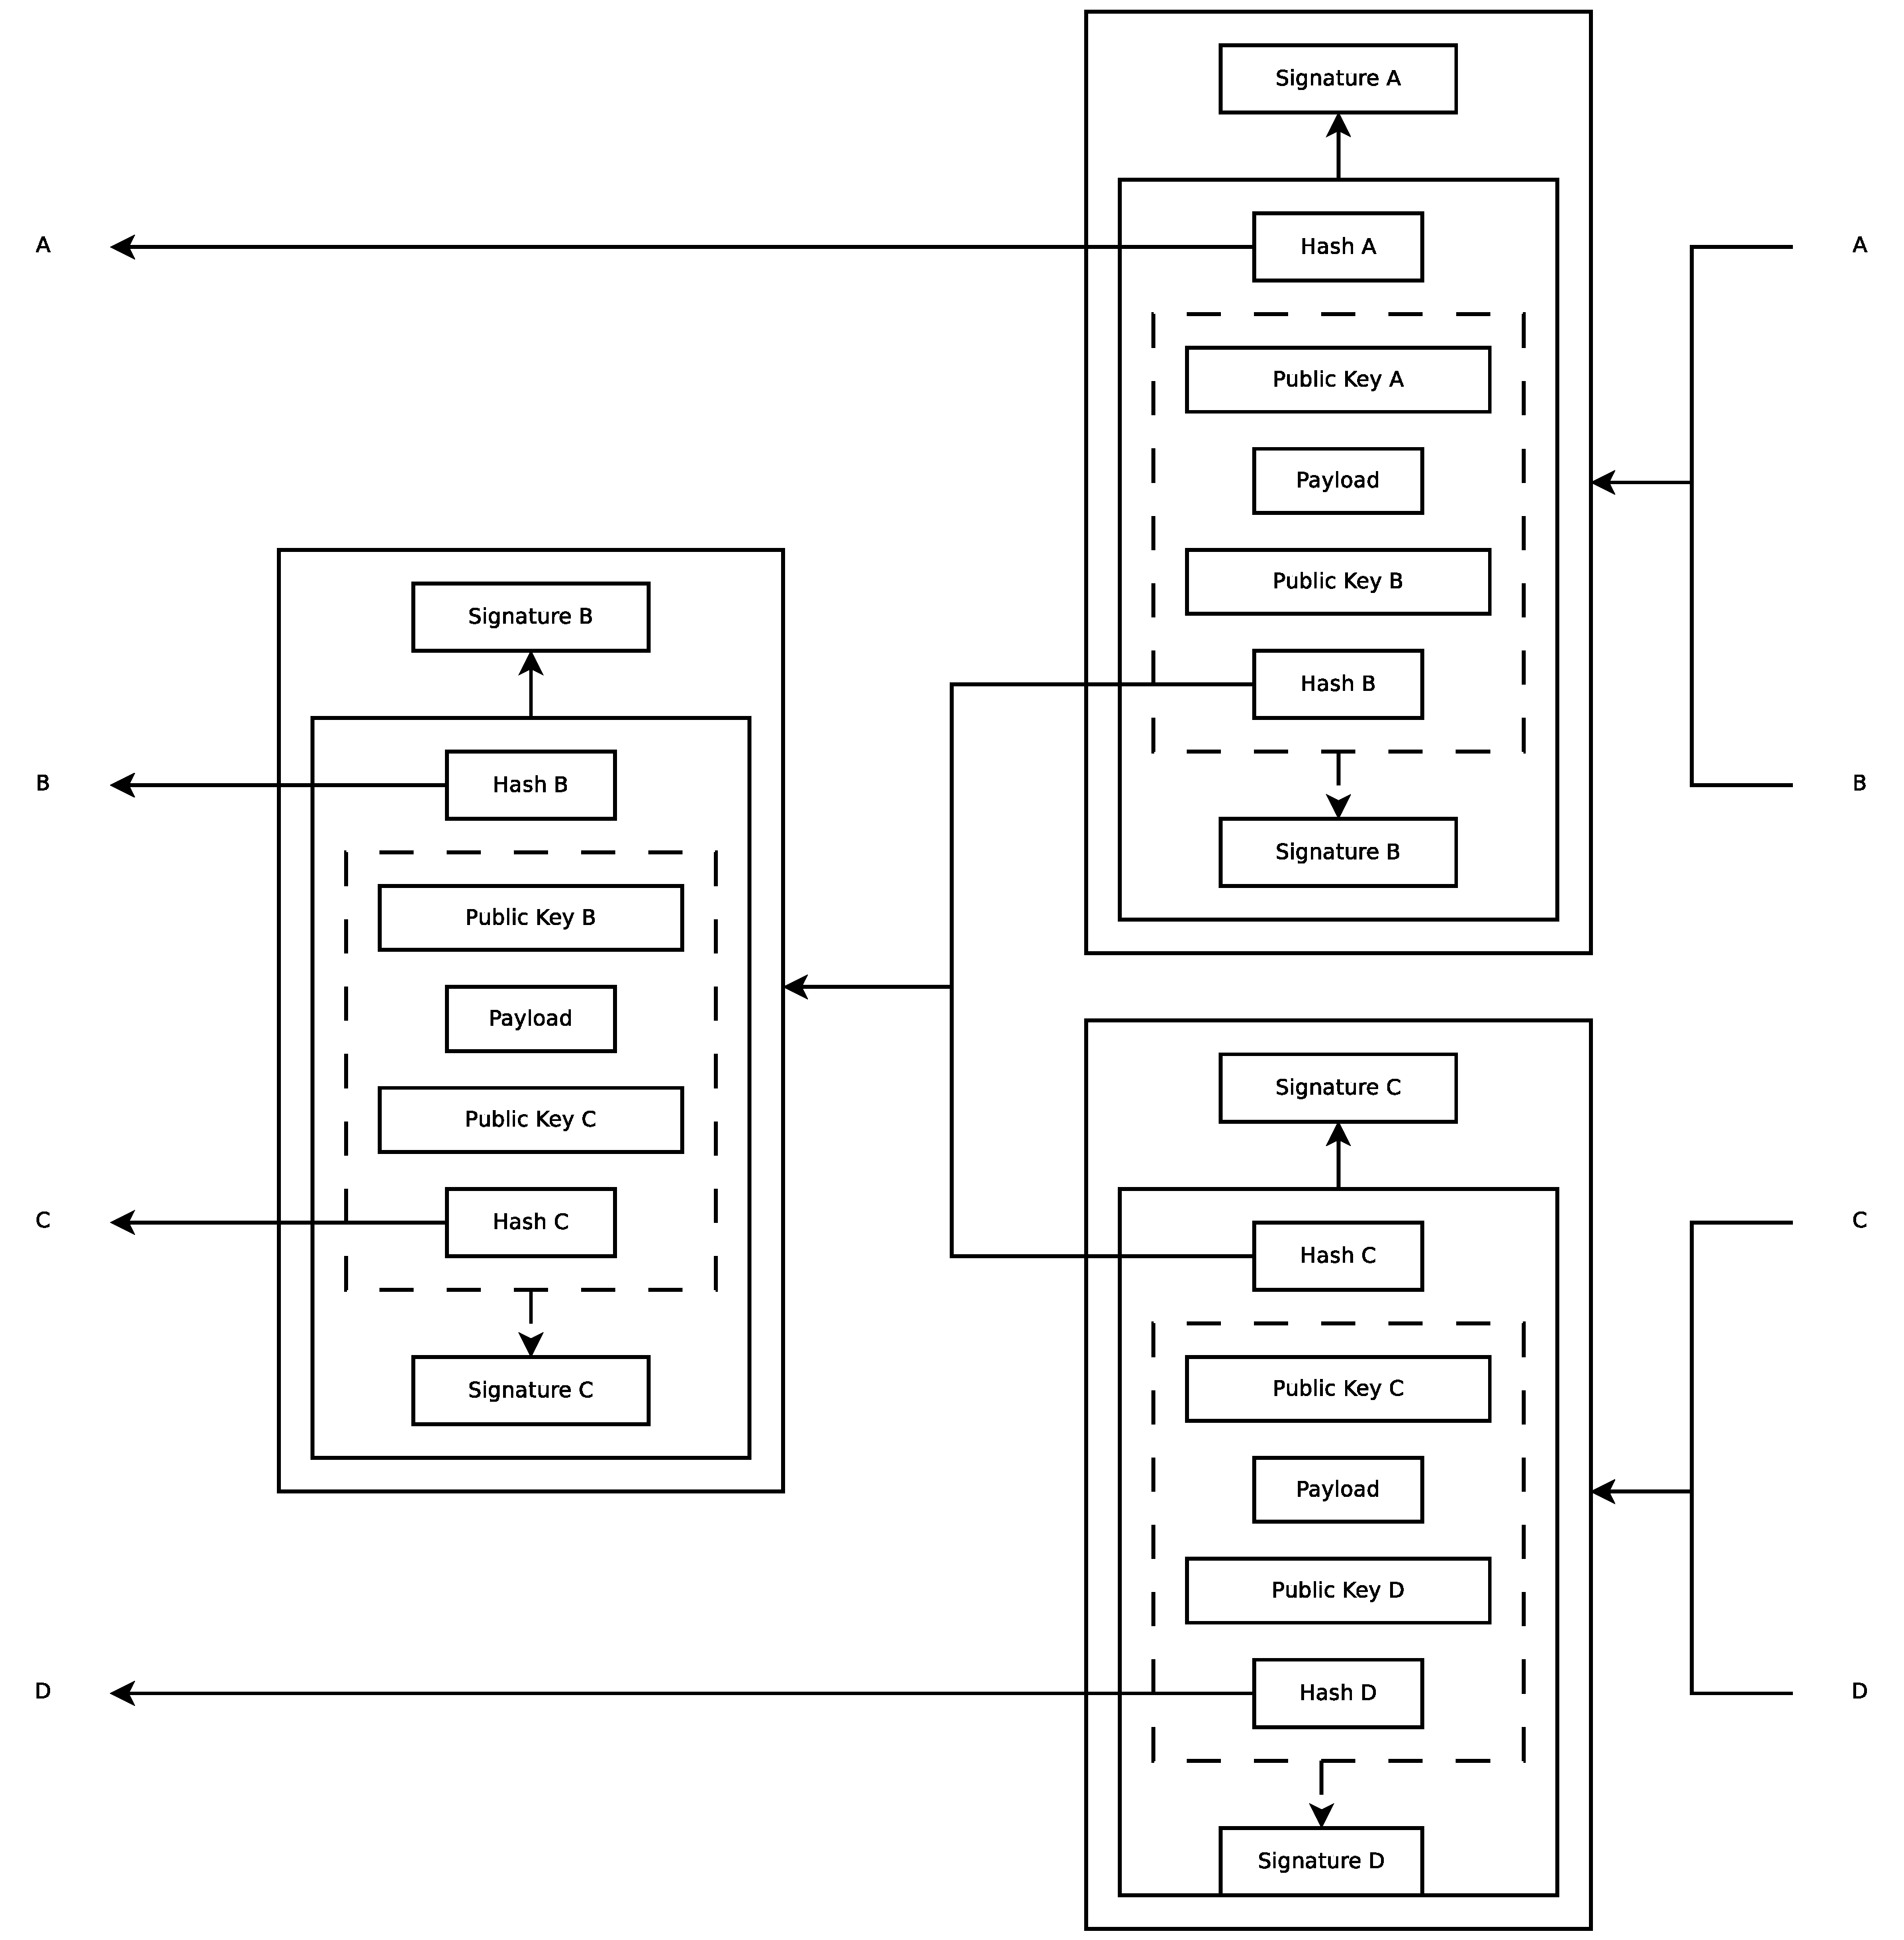
\includegraphics[scale=0.3]{design/figs/chain.eps}}
	\caption{Example of three blocks in the chain.}
	\label{fig:chain-example}
\end{figure}